	\documentclass[]{beamer}
 
\usepackage[utf8]{inputenc} 
\usepackage[T1]{fontenc}
\usepackage{lmodern}
\usepackage{graphicx}
\usepackage[french]{babel}
\usepackage{tikz}
\usepackage{listings}
 %\useoutertheme[subsection=false]{smoothbars}


\usetheme{Warsaw}
%\usetheme{Madrid}
%\usetheme{Frankfurt}
\setbeamertemplate{navigation symbols}{\insertframenumber/\,\inserttotalframenumber}

\begin{document}
 %\hspace*{1cm} \insertframenumber\,/\,\inserttotalframenumber
\title[Inférence de la structure d'une page web]{Inférence de la structure d'une page web en vue d'améliorer son accessibilité}
\subtitle[\ldots]{Encadré par : Y. Bonavero, M. Huchard et M. Meynard}
\author[Franck PETITDEMANGE]{Franck PETITDEMANGE}
\institute[LIRMM]{
\includegraphics[scale=0.2]{img/logo-lirmm.jpg}\hspace{2cm}
\includegraphics[scale=0.3]{img/logo-cnrs.jpg}}
\date{26 juin 2014}
%\setbeamertemplate{footline}[page number]




\begin{frame}
\titlepage
\end{frame}

\begin{frame}
  \frametitle{Sommaire}
  \tableofcontents[hideothersubsections]
\end{frame}

\section{Introduction} 
\begin{frame}
  \frametitle{Sommaire}
  \tableofcontents[currentsection, hideothersubsections]
\end{frame}

\begin{frame}
	\frametitle{Accessibilité du web}
	\framesubtitle{Un enjeux sociétale important}
	\begin{definition}{Accessibilité}
	Capacité d'accéder aux informations contenues dans une page et d'interagir avec.
	\end{definition}
	\begin{block}{Problèmes d'accessibilité (spécifique aux basses visions)}
		\begin{itemize}
			\item Surcharge visuelle
			\item Police de caractère
			\item Contraste de couleur
		\end{itemize}
	\end{block}
\end{frame}

\begin{frame}
\frametitle{Accessibilité du web}
\framesubtitle{Besoin de comprendre la structuration d'une page}
	%\begin{columns}
	%\begin{column}{5cm}
	\begin{block}{Problèmes des outils accessibilité}
	\begin{itemize}
		\item Pas de traitement des couleurs locales
		\item Pas de prise en compte des profils utilisateurs
	\end{itemize}
	\end{block}
	\begin{block}{Besoin}
	\begin{itemize}
		\item Comprendre les informations structurant une page web
	\end{itemize}
	\end{block}
	%\end{column}
	%\begin{column}{5cm}
	%\fbox{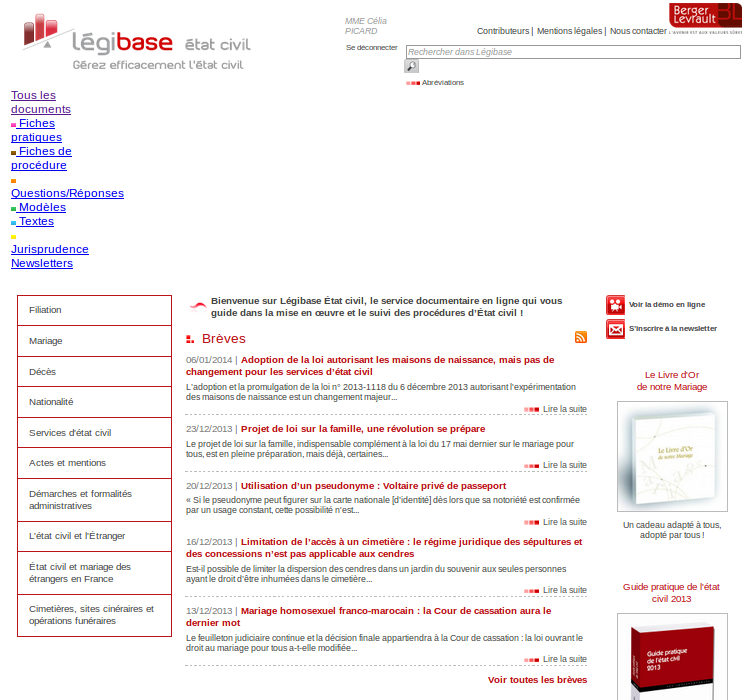
\includegraphics[scale=0.2]{img/page_berger.png}}
	%\end{column}
	%\end{columns}
\end{frame}



\begin{frame}
	\frametitle{Page web}
	\begin{columns}
	\begin{column}{5cm}
		\begin{block}{Page web}
		\begin{itemize}
			\item Technologies : HTML/CSS/Javascript
			\item Contenu hétérogène décrit par différentes structures logiques
		\end{itemize}
		\end{block}
		%\begin{block}{}
		%\end{block}
	\end{column}
	\begin{column}{5cm}
	\fbox{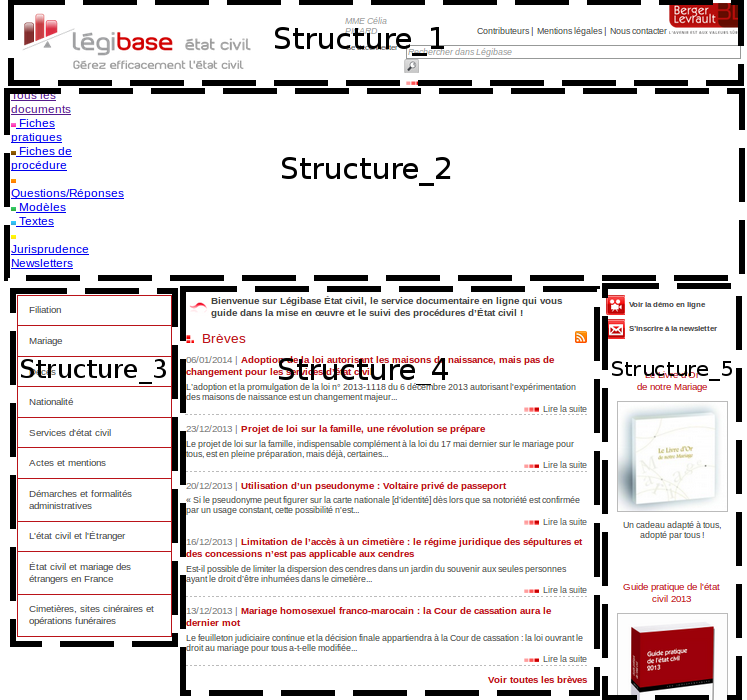
\includegraphics[scale=0.2]{img/segmentation_page_berger.png}}
	\end{column}
	\end{columns}
\end{frame}

\begin{frame}
	\frametitle{}
	\begin{block}{}
	Comment inférer les différentes structures logiques dans une page web?
	\end{block}
	\begin{block}{Difficultés}
		\begin{itemize}
			\item Manque d'expressivité de HTML 4
			\item Pas de construction standard des structures logiques
			%\item Syntaxe de HTML 4 autorise des constructions non conformes au W3C
			\item Écart entre la structure DOM et l'affichage dans un navigateur
		\end{itemize}
	\end{block}
	\begin{block}{Approche}
		\begin{itemize}
			\item Étude des langages de publication de page web
			\item Étude des techniques d'extraction de structure d'une page
		\end{itemize}
	\end{block}
\end{frame}


\section{État de l'art}

\begin{frame}
  \frametitle{Sommaire}
  \tableofcontents[currentsection, hideothersubsections]
\end{frame}

\subsection{Étude des Langages de publication}
\begin{frame}[fragile]
\frametitle{Évolution de la sémantique (1/2)}
\begin{columns}
	\begin{column}{5cm}
\begin{lstlisting}[frame=single, language=html]
<ul class='menu'>
 <li><a href=".">l1</li>
 <li><a href=".">l2</li>
</ul>
<p class='menu'>
 <a href=".">l1</a>
 <a href=".">li2</a>
</p>
\end{lstlisting}
	\end{column}
	\begin{column}{5cm}
	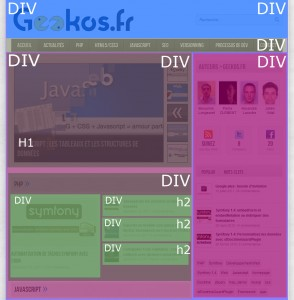
\includegraphics[scale=0.4]{img/architecture_HTML4.jpg}	
	\end{column}
\end{columns}
	\begin{block}{HTML 4}
	\begin{itemize}
		\item Peu de sémantique
		\item Structure générique (DIV)
		\item Structure logique implicite
	\end{itemize}
	\end{block}
\end{frame}

\begin{frame}
\frametitle{Évolution de la sémantique (2/2)}
\begin{columns}
	\begin{column}{5cm}
	\begin{block}{HTML 5}
		\begin{itemize}
			\item Structure logique explicitée
			\item Sémantique pour décrire l'interface de la page est limitée
		\end{itemize}
	\end{block}
	\begin{block}{ARIA}
		\begin{itemize}
			\item Ontologie d'une interface graphique
			\item Trop élaborée pour nos besoins mais est plus expressif
		\end{itemize}
	\end{block}
	\end{column}
	\begin{column}{5cm}
	\temporal<2->{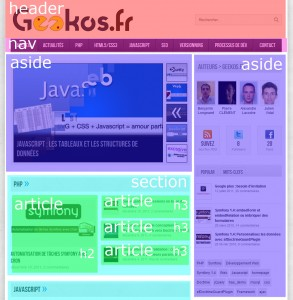
\includegraphics[scale=0.5]{img/architecture_HTML5.jpg}}{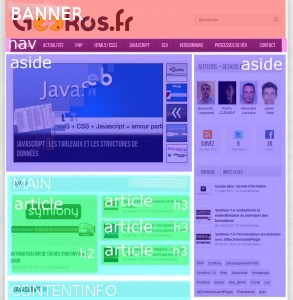
\includegraphics[scale=0.5]{img/architecture_ARIA.jpg}}
	
	\end{column}
\end{columns}
\end{frame}


\begin{frame}
\frametitle{CSS}
\framesubtitle{Un langage de mise en forme}
\begin{columns}
	\begin{column}{5cm}
	\begin{block}{Propriétés de mise en forme :}		
		\begin{itemize}
			\item avant-plan/arrière-plan
			\item police
			\item ...
		\end{itemize}
	\end{block}
	\begin{block}{Mécanisme de positionnement}
		\begin{itemize}
			\item relatif
			\item absolu
			\item flottant
		\end{itemize}
	\end{block}
	\end{column}
	\begin{column}{5cm}
	\end{column}
\end{columns}\end{frame}

\begin{frame}
\frametitle{Synthèse}
\begin{block}{}
HTML 4 langage actuellement le plus exploité. Les inconvénients sont :
\begin{itemize}
	\item la diversité de représentation d'une même structure logique
	\item la faible expressivité au regard des concepts décrits dans les pages web
\end{itemize}
\end{block}
\begin{block}{Notre approche}
\begin{itemize}
	\item Proposer un Méta-modèle concrétisant mieux les concepts des pages et permettant de s'abstraire de la diversité de représentation des structures 
\end{itemize}
\end{block}
\end{frame}

\subsection{Étude de méthodes d'extraction de structure}
\begin{frame}
\frametitle{Mapping}
\framesubtitle{\textit{(Vieira et al., A fast and robust method for web page template detection and removal)}}
\begin{columns}
	\begin{column}{5cm}
	\begin{block}{Mapping descendant restrictif}
		Permet de faire correspondre les plus grandes sous-structures communes entre deux arbres
	\end{block}
	\begin{block}{Idée}
		Identifier les structures logiques des pages web par correspondance
	\end{block}
	\end{column}
	\begin{column}{5cm}
		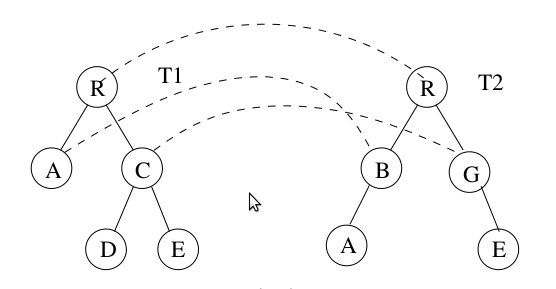
\includegraphics[scale=0.3]{img/mapping.jpg}
	\end{column}
\end{columns}
\end{frame}

\begin{frame}
\frametitle{Segmentation}
\framesubtitle{par pattern de présentation \textit{(Milos Kovacevic et al., Recognition of Common Areas in a Web Page Using Visual Information: a possible application in a page classification)}}
\begin{columns}
	\begin{column}{5cm}
	\begin{block}{Observation}
		Les concepteurs de page web suivent approximativement les mêmes schémas de présentation
	\end{block}
	\begin{block}{Idée}
		Regrouper les n\oe{}uds du DOM de la page suivant leurs coordonnées après la mise en page par le navigateur
	\end{block}
	\end{column}
	\begin{column}{5cm}
		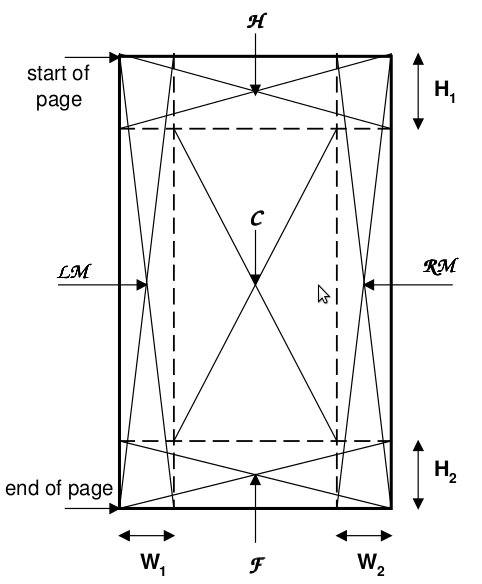
\includegraphics[scale=0.3]{img/segmentation-pattern.jpg}
	\end{column}
\end{columns}
\end{frame}

\begin{frame}
\frametitle{Segmentation}
\framesubtitle{par densitométrie textuelle \textit{(Kohlsch{\"u}tter et al, A densitometric approach to web page segmentation)}}

\begin{block}{Étape 1 : identification de segments de petites tailles}	
La page est vue comme une séquences de caractères entrelacés identifiés par des balises HTML. Les segments sont calculés d'après les variations dans le rythme des séquences.\\
Exemple : \\
Ici deux segments seront calculés \\
\textit{<a>lien</a>lien<a>lien</a><p>un paragraphe</p>}
\end{block}

\begin{block}{Étape 2 : grossissement successif des segments par fusion}
Les segments contingents dont la densité textuelle est proche sont fusionnées successivement.
\end{block}

\end{frame}

\begin{frame}
\frametitle{Segmentation}
\framesubtitle{par indice visuel \textit{(Cai et al., Extracting content structure for web pages based on visual representation)}}
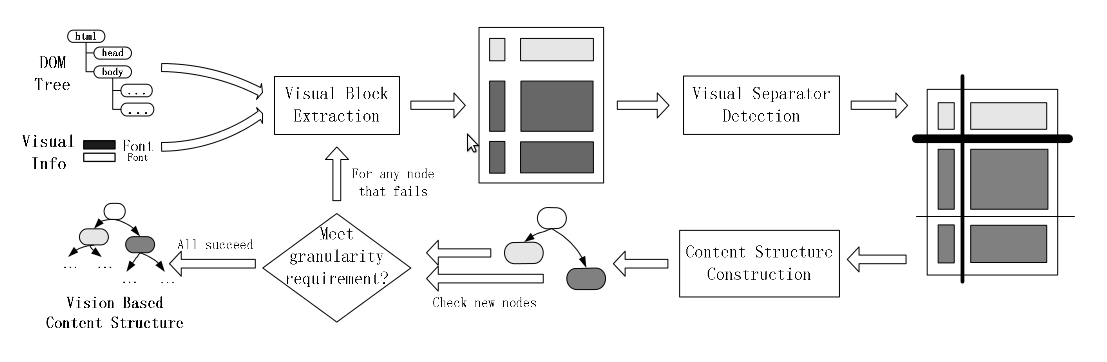
\includegraphics[scale=0.3]{img/segmentation-vips.png}
\end{frame}

\begin{frame}
\frametitle{Synthèse}
\begin{block}{Les inconvénients}
	\begin{itemize}
		\item Mapping ne permet pas d'extraire la structure globale de la page
		\item La segmentation par pattern est trop dépendante de la présentation de la page
		\item La segmentation par densitométrie ne prend pas en compte les écarts possible entre le DOM et le rendu final
		\item Le calcule des séparateurs dans l'approche par indice visuel est une opération coûteuse $O(n^2)$
	\end{itemize}
\end{block}
\begin{block}{Notre approche : approche par segmentation par visuel}
Propose un \textbf{découpage globale} de la page, \textbf{indépendant des patterns de présentation} et permet un \textbf{découpage fin} dans la structure d'une page.
\end{block}
\end{frame}

\section{Réalisation}
\begin{frame}
  \frametitle{Sommaire}
  \tableofcontents[currentsection, hideothersubsections]
\end{frame}

\subsection{Méta-modèle}

\begin{frame}
	\frametitle{Approche générale}
	\framesubtitle{Une approche Ingénierie Dirigée par les Modèles}
	\begin{columns}
		\begin{column}{4cm}
			\begin{block}{Avantages}
				\begin{itemize}
					\item Meilleur expression des préférences
					\item Indépendant de la diversité de représentation des informations
				\end{itemize}
			\end{block}
		\end{column}
		\begin{column}{6cm}
		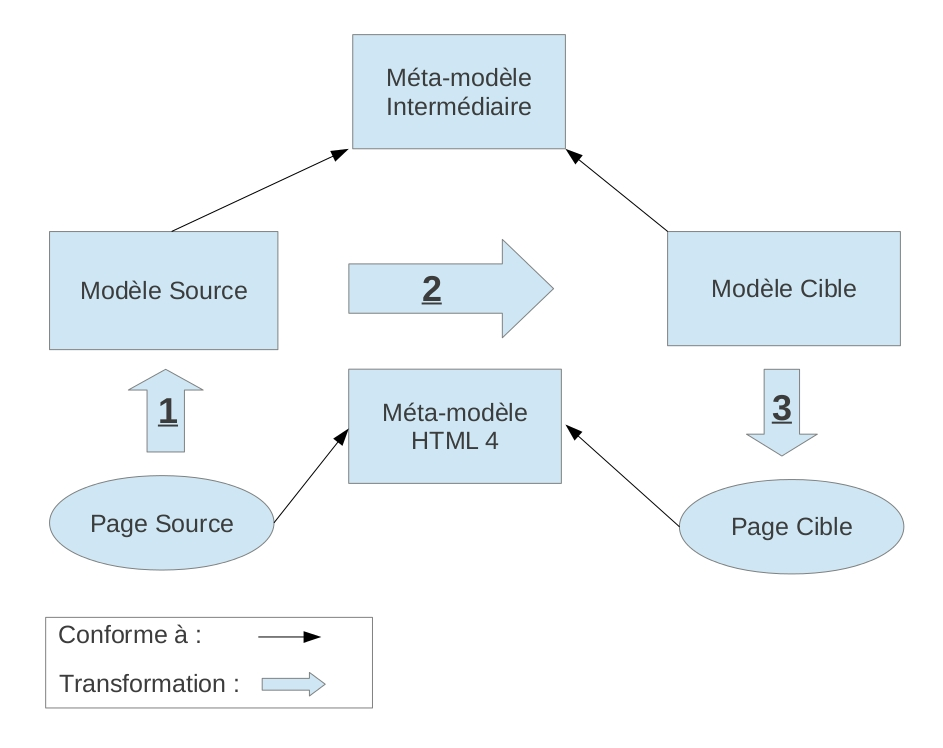
\includegraphics[scale=0.3]{img/workflow-adaptation.jpg}
		\end{column}		
	\end{columns}
\end{frame}






\begin{frame}
\frametitle{Méta-modèle intermédiaire}
\framesubtitle{Éléments structurels}
\begin{figure}
\centering
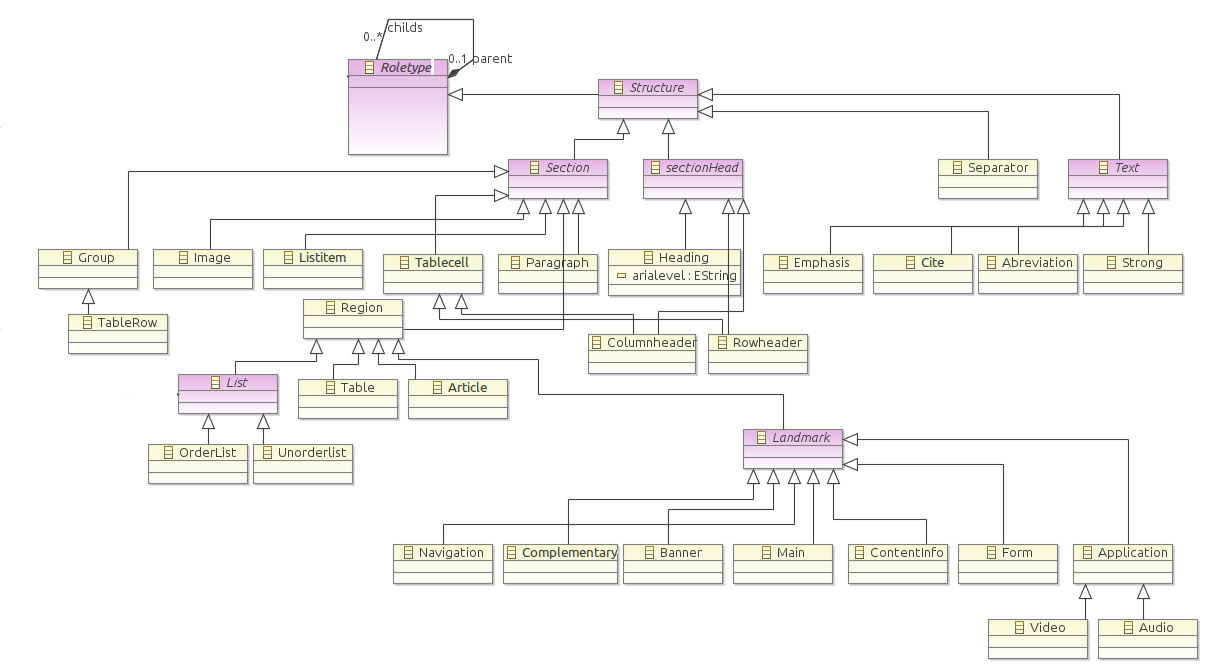
\includegraphics[scale=0.335]{img/metamodele_structure.png}
\end{figure}
\end{frame}

\begin{frame}
\frametitle{Méta-modèle intermédiaire}
\framesubtitle{Éléments d'interaction}
\begin{figure}
\centering
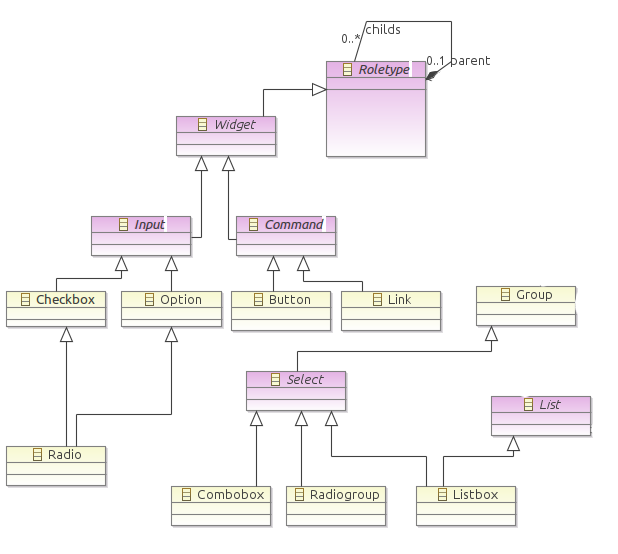
\includegraphics[scale=0.4]{img/metamodele_widget.png}
\end{figure}
\end{frame}

\begin{frame}
\frametitle{Méta-modèle intermédiaire}
\framesubtitle{Éléments de mise en forme}
\begin{figure}
\centering
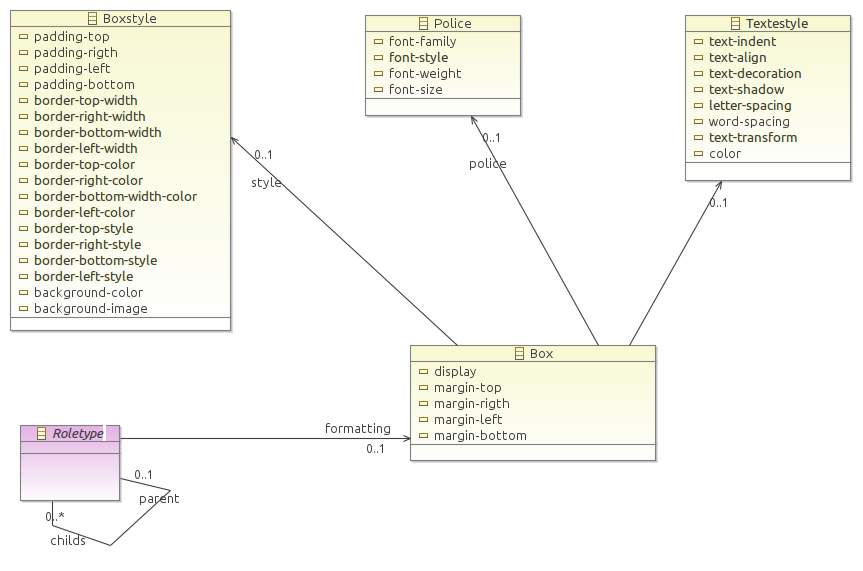
\includegraphics[scale=0.4]{img/metamodele_CSS.png}
\end{figure}
\end{frame}

\subsection{Extraction structure}
\begin{frame}
\frametitle{Démarche générale}
\end{frame}

\begin{frame}
\frametitle{Concepts et heuristiques}
\end{frame}
\subsection{Annotation structure}
\begin{frame}
\frametitle{Approche par fonctionnalité}
\framesubtitle{Modèle orientée fonctionnalité}
\end{frame}

\begin{frame}
\frametitle{Approche par fonctionnalité}
\framesubtitle{fonctions de détection proposées}
\end{frame}


\begin{frame}
	\frametitle{Processus d'extraction}
	\framesubtitle{Segmentation globale page Berger-Levrault}
\end{frame}

\begin{frame}
	\frametitle{Processus d'extraction}
	\framesubtitle{Segmentation locale page Berger-Levrault}
\end{frame}


\section{Conclusion}
\begin{frame}
  \frametitle{Sommaire}
  \tableofcontents[currentsection, hideothersubsections]
\end{frame}
\subsection{Résultats}
\begin{frame}
	\frametitle{Résultats}
	\begin{block}{Résultats}
		\begin{itemize}
			\item Proposition d'une approche IDM  
			\item État de l'art sur les langages de publication de page web
			\item État de l'art des techniques d'extraction de structure
			\item Proposition d'un méta-modèle
			\item Adaptation et implémentation d'une méthode pour extraire les structures d'une page
			\item Proposition de pistes pour annoter les structures extraites  
		\end{itemize}
	\end{block}
\end{frame}

\subsection{Difficultés et perspectives}
\begin{frame}
	\frametitle{Difficultés et perspectives}
	\begin{block}{Difficultés}
		\begin{itemize}
			\item Domaine de recherche éloigné des connaissances de l'équipe de recherche
			\item Définir la problématique par rapport à la question de recherche (recherche de motifs d'intérêt dans un arbre DOM)
			\item Recherche d'articles traitant de la problématique
		\end{itemize}
	\end{block}
	\begin{block}{Perspectives}
		\begin{itemize}
			\item Évaluation de la méthode d'extraction de structure
			\item Implémentation, évaluation et élargissement du processus d'annotation
		\end{itemize}
	\end{block}
\end{frame}
 
\end{document}